\def\figpath{tex/5_Differenzverstaerker/pictures}
\graphicspath{{tex/5_Differenzverstaerker/pictures/}}

\chapter{Differenzverstärker}
In Kapitel 5 werden die Eigenschaften einer einfachen und einer erweiterten Differenzverstärkerschaltung untersucht.

\section{Einfacher Differenzverstärker}
Abb. \ref{} zeigt das Ersatzschaltbild eines einfachen Differenzverstärkers mit einem einzigen Ausgang. 

\begin{figure}[H]
	\centering
	\def\svgwidth{0.7\textwidth}
	\input{\figpath/DiffVerstärker.pdf_tex}
	\caption{Einfacher Differenzverstärker} 
	\label{fig_Kap5_01:ESBDiffVerst} 
\end{figure}

\subsection{Dimensionierung der Kollektorwiderstände $R_C$}

Im ersten Schritt müssen die Kollektorwiderstände dermaßen dimensioniert werden, so dass die Kollektorpotentiale, im Arbeitspunkt $U_P = U_N = \SI{0}{\volt}$, auf \SI{7.5}{\volt} liegen. Die Emitterwiderstände sollen \SI{33}{\ohm} betragen.

Der Strom der Stromquelle von \SI{10}{\milli \ampere} teilt sich gleichmäßig auf die Beiden Kollektorströme ($I_{c1} = I_{c2} = I_c$ auf (Basisströme werden gerechtfertigterweise vernachlässigt). Der Strom durch die Kollektorwiderstände beträgt also jeweils \SI{5}{\milli \ampere} und an den beiden Widerständen soll \SI{7.5}{\volt} abfallen. Dies liefert über das ohmsche Gesetz den gesuchten Widerstandswert:

\begin{equation}
    V_c = \SI{7.5}{\volt} = \SI{15}{\volt} - R_c I_c \rightarrow Rc = \frac{\SI{7.5}{\volt} - \SI{15}{\volt}}{- I_c} = \SI{1.5}{\kilo \ohm}
\end{equation}

\subsection{Kleinsignal-Spannungsverstärkung $A_{ed}$}
Im nächsten Schritt soll die Kleinsignal-Spannungsverstärkung nach

\begin{equation}
    A_{ed} = \frac{u_A}{u_P - u_N}
\end{equation}

für die Fälle $R_E = \SI{0}{\ohm}$ und $R_E = \SI{33}{\ohm}$berechnet und simuliert werden. Dafür wird zunächst das KSESB betrachtet, siehe Abb. \ref{fig_Kap5_02:ESBDiffVerstKSBES}.

\begin{figure}[H]
	\centering
	\def\svgwidth{0.9\textwidth}
	\input{\figpath/DiffVerstärker_1_KSESB.pdf_tex}
	\caption{Einfacher Differenzverstärker KSESB} 
	\label{fig_Kap5_02:ESBDiffVerstKSBES} 
\end{figure}

Des Weiteren soll es sich hier um eine schiefsymmetrische Aussteuerung handeln, sprich

\begin{equation}
    u_P = -u_N = u_E
\end{equation}

\begin{equation}
    \label{Gln_I}
    u_P = i{B,1} ( \frac{B}{S} + R_E\cdot (B + 1) ) + R_i \cdot (B+1)(i{B,1} + i{B,2}) = u_E
\end{equation}

\begin{equation}
    \label{Gln_II}
    u_N = i{B,2} ( \frac{B}{S} + R_E\cdot (B + 1) ) + R_i \cdot (B+1)(i{B,1} + i{B,2}) = -u_E
\end{equation}

Subtrahiert man beide Gleichungen voneinander, erhält man

\begin{equation}
    i_{B,1} \cdot \left( -\frac{B}{S} - R_E(B+1) - 2R_i(B+1) \right) = i_{B,2} \cdot \left( +\frac{B}{S} + R_E(B+1) + 2R_i(B+1) \right)
\end{equation}

\begin{equation}
    \label{current}
    i_{B,1} = -i_{B,2}
\end{equation}

Für die Ausgangsspannung gilt

\begin{equation}
    u_a = -R_C B i_{B,2} = R_C B i_{B,1}
\end{equation}

Legt man eine Maschen von $u_P$ bis $u_N$ gelangt man zum Zusammenhang

\begin{equation}
    u_P = \left( \frac{B}{S} + R_E(B+1) \right) (i_{B,1} - i_{B,2} ) + u_N, 
\end{equation}

woraus folgt dass mit Glng. \ref{current} gilt

\begin{equation}
    u_P - u_N = 2i_{B,1} \left( \frac{B}{S} + R_E(B+1) \right)
\end{equation}

Setzt man dies in Glng. 5.2 ein, so erhält man für die Differenzverstärkung

\begin{equation}
    A_{ed} = \frac{R_C B i_{B,1}}{2i_{B,1} \left( \frac{B}{S} + R_E(B+1) \right)} = \frac{R_C S}{2\left( 1 + R_E S(1+\frac{1}{B}) \right)} \approx \frac{R_C S}{2\left( 1 + R_E S \right)}
\end{equation}

Für die in Tab. \ref{tab_Kap5_01:Bauteilwerte} angeführten Parameter gilt lässt sich die Differenzverstärkung berechnen.

\begin{table}[H]
\centering
\begin{tabular}{|c|c|} \hline
Benennung & Größe \\ \hline
$R_C$ & \SI{1500}{\ohm} \\ \hline
$I_{C,0}$ & \SI{5}{\milli\ampere} \\ \hline
$B$ & 290 \\ \hline
$U_T$ & \SI{25,9}{\milli\volt} \\ \hline
\end{tabular}
\caption{Parameter für Berechnung und Simulation}
\label{tab_Kap5_01:Bauteilwerte} 
\end{table}

Für einen Emitterwiderstand von $R_E = \SI{33}{\ohm}$ gilt somit

\begin{equation}
    A_{ed} = \frac{R_C S}{2\left( 1 + R_E S(1+\frac{1}{B}) \right)} = \frac{\SI{1500}{\ohm}\cdot\SI{0,2}{\ampere\per\volt}}{2(1+\SI{33}{\ohm} \cdot \SI{0,2}{\ampere\per\volt} (1 + \frac{1}{290}) )} = 19.68 \hat{=} 25.88\text{dB} .
\end{equation}

Für einen Emitterwiderstand von $R_E = \SI{0}{\ohm}$ gilt dagegen

\begin{equation}
    A_{ed} = \frac{R_C S}{2} =  \frac{\SI{1500}{\ohm}\cdot\SI{0,2}{\ampere\per\volt}}{2} = 150 \hat{=} 43.5\text{dB} .
\end{equation}

Nun wird die Kleinsignalverstärkung simuliert, siehe Abb. \ref{fig_Kap5_03:SpiceSchematic}.

\begin{figure}[H]
    \centering
    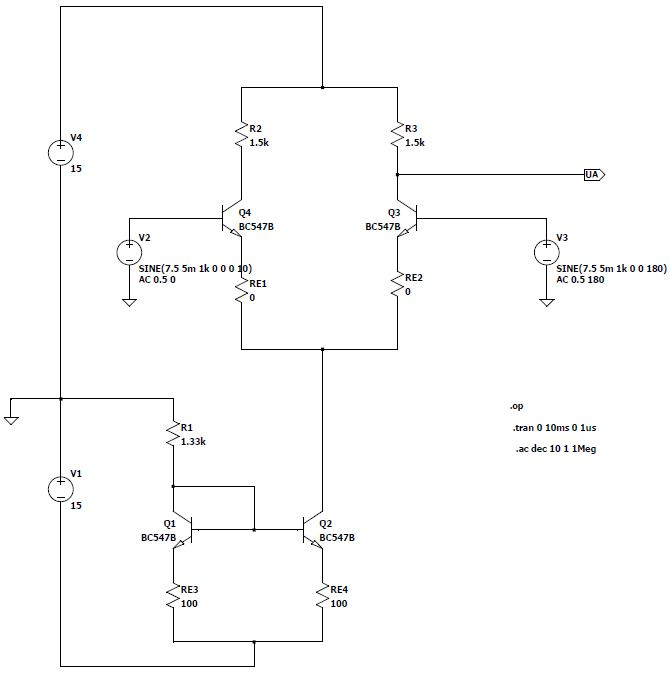
\includegraphics[width = 0.6\textwidth]{\figpath/einfachDiff.jpg}
    \caption{Einfacher Stromspiegel in LTSpice}
    \label{fig_Kap5_03:SpiceSchematic}
\end{figure}

Mit einer AC-Analyse kann das Bode-Diagramm und daraus die Verstärkung abgelesen werden. Mit $R_E = \SI{0}{\ohm}$ wird eine Verstärkung von 

\begin{equation}
    A_{ed} = 41.17\text{dB} \hat{=} 114.4
\end{equation}

simuliert. Mit $R_E = \SI{33}{\ohm}$ wird hingegen eine Verstärkung von 

\begin{equation}
    A_{ed} = 25.5\text{dB} \hat{=} 18.8
\end{equation}

erreicht. Die Verstärkung bei $R_E = \SI{0}{\ohm}$ weicht doch beträchtlich vom berechneten Wert ab.

\begin{figure}[H]
	\centering \small
	\scalebox{0.9}{% This file was created by matlab2tikz.
%
\definecolor{mycolor1}{rgb}{0.00000,0.44700,0.74100}%
\definecolor{mycolor2}{rgb}{0.85000,0.32500,0.09800}%
%
\begin{tikzpicture}

\begin{axis}[%
width=4.521in,
height=3.566in,
at={(0.758in,0.481in)},
scale only axis,
xmode=log,
xmin=1,
xmax=100000000,
xminorticks=true,
xlabel style={font=\color{white!15!black}},
xlabel={$f \text{ in } \text{Hz}$},
ymin=10,
ymax=45,
ylabel style={font=\color{white!15!black}},
ylabel={$A_{ed} \text{ in } \text{dB}$},
axis background/.style={fill=white},
title style={font=\bfseries},
title={$A_{ed}$},
xmajorgrids,
xminorgrids,
ymajorgrids,
legend style={at={(0.03,0.03)}, anchor=south west, legend cell align=left, align=left, draw=white!15!black}
]
\addplot [color=mycolor1]
  table[row sep=crcr]{%
1	41.1675597085499\\
1.25892541179417	41.1675597085499\\
1.58489319246111	41.1675597085499\\
1.99526231496888	41.1675597085499\\
2.51188643150958	41.1675597085499\\
3.16227766016838	41.1675597085499\\
3.98107170553497	41.1675597085499\\
5.01187233627272	41.1675597085498\\
6.30957344480194	41.1675597085497\\
7.94328234724282	41.1675597085496\\
10	41.1675597085494\\
12.5892541179417	41.1675597085491\\
15.8489319246111	41.1675597085486\\
19.9526231496888	41.1675597085478\\
25.1188643150958	41.1675597085466\\
31.6227766016838	41.1675597085447\\
39.8107170553498	41.1675597085416\\
50.1187233627273	41.1675597085367\\
63.0957344480194	41.167559708529\\
79.4328234724283	41.1675597085168\\
100	41.1675597084974\\
125.892541179417	41.1675597084666\\
158.489319246112	41.1675597084179\\
199.526231496888	41.1675597083407\\
251.188643150958	41.1675597082183\\
316.227766016838	41.1675597080244\\
398.107170553498	41.1675597077169\\
501.187233627273	41.1675597072297\\
630.957344480194	41.1675597064575\\
794.328234724283	41.1675597052337\\
1000	41.1675597032941\\
1258.92541179417	41.16755970022\\
1584.89319246112	41.1675596953478\\
1995.26231496888	41.167559687626\\
2511.88643150959	41.1675596753877\\
3162.27766016839	41.1675596559913\\
3981.07170553498	41.1675596252502\\
5011.87233627273	41.1675595765287\\
6309.57344480195	41.1675594993104\\
7943.28234724283	41.1675593769276\\
10000	41.167559182964\\
12589.2541179417	41.1675588755524\\
15848.9319246112	41.1675583883378\\
19952.6231496889	41.1675576161549\\
25118.8643150959	41.1675563923278\\
31622.7766016839	41.1675544526933\\
39810.7170553498	41.1675513785814\\
50118.7233627274	41.1675465064469\\
63095.7344480195	41.1675387846453\\
79432.8234724284	41.1675265464426\\
100000	41.1675071502689\\
125892.541179417	41.1674764095824\\
158489.319246112	41.1674276893225\\
199526.231496889	41.1673504740319\\
251188.643150959	41.1672280988505\\
316227.766016839	41.1670341543093\\
398107.170553499	41.166726790635\\
501187.233627274	41.1662396965157\\
630957.344480196	41.1654678160529\\
794328.234724285	41.1642447484103\\
1000000	41.1623070208594\\
1258925.41179417	41.1592376964086\\
1584893.19246112	41.1543775761543\\
1995262.31496889	41.1466859086149\\
2511886.43150959	41.1345232234583\\
3162277.66016839	41.1153160457674\\
3981071.70553499	41.0850473530381\\
5011872.33627275	41.0375019329754\\
6309573.44480196	40.9631958938044\\
7943282.34724285	40.8479680048281\\
10000000	40.6713734757856\\
12589254.1179417	40.4053899925528\\
15848931.9246112	40.0145448431442\\
19952623.1496889	39.4590867279285\\
25118864.3150959	38.7023186825246\\
31622776.6016839	37.7206902592622\\
39810717.0553499	36.5118028909646\\
50118723.3627275	35.0950901786693\\
63095734.4480196	33.5046166915506\\
79432823.4724286	31.7787008679182\\
100000000	29.9515824393383\\
};
\addlegendentry{$R_E = \SI{0}{\ohm}$}

\addplot [color=mycolor2]
  table[row sep=crcr]{%
1	25.5228956217106\\
1.25892541179417	25.5228956217106\\
1.58489319246111	25.5228956217106\\
1.99526231496888	25.5228956217106\\
2.51188643150958	25.5228956217106\\
3.16227766016838	25.5228956217106\\
3.98107170553497	25.5228956217105\\
5.01187233627272	25.5228956217104\\
6.30957344480194	25.5228956217103\\
7.94328234724282	25.5228956217102\\
10	25.52289562171\\
12.5892541179417	25.5228956217097\\
15.8489319246111	25.5228956217091\\
19.9526231496888	25.5228956217083\\
25.1188643150958	25.522895621707\\
31.6227766016838	25.5228956217053\\
39.8107170553498	25.522895621702\\
50.1187233627273	25.5228956216969\\
63.0957344480194	25.5228956216888\\
79.4328234724283	25.5228956216764\\
100	25.5228956216565\\
125.892541179417	25.5228956216246\\
158.489319246112	25.5228956215747\\
199.526231496888	25.522895621495\\
251.188643150958	25.5228956213689\\
316.227766016838	25.5228956211692\\
398.107170553498	25.5228956208526\\
501.187233627273	25.5228956203507\\
630.957344480194	25.5228956195553\\
794.328234724283	25.5228956182946\\
1000	25.5228956162967\\
1258.92541179417	25.5228956131303\\
1584.89319246112	25.5228956081119\\
1995.26231496888	25.522895600158\\
2511.88643150959	25.5228955875521\\
3162.27766016839	25.522895567573\\
3981.07170553498	25.5228955359085\\
5011.87233627273	25.5228954857234\\
6309.57344480195	25.5228954061853\\
7943.28234724283	25.5228952801263\\
10000	25.5228950803359\\
12589.2541179417	25.5228947636896\\
15848.9319246112	25.5228942618392\\
19952.6231496889	25.5228934664598\\
25118.8643150959	25.5228922058687\\
31622.7766016839	25.5228902079673\\
39810.7170553498	25.5228870415087\\
50118.7233627274	25.5228820230149\\
63095.7344480195	25.5228740692496\\
79432.8234724284	25.5228614634109\\
100000	25.5228414845765\\
125892.541179417	25.5228098204432\\
158489.319246112	25.5227596366393\\
199526.231496889	25.522680101839\\
251188.643150959	25.5225540506117\\
316227.766016839	25.5223542802543\\
398107.170553499	25.5220376840981\\
501187.233627274	25.521535959526\\
630957.344480196	25.5207408964931\\
794328.234724285	25.5194810998442\\
1000000	25.5174851930922\\
1258925.41179417	25.5143237419672\\
1584893.19246112	25.5093178141362\\
1995262.31496889	25.50139556614\\
2511886.43150959	25.4888687067873\\
3162277.66016839	25.4690875162491\\
3981071.70553499	25.4379169103328\\
5011872.33627275	25.388961299833\\
6309573.44480196	25.3124669298499\\
7943282.34724285	25.1938817442867\\
10000000	25.0122223881563\\
12589254.1179417	24.7387772969232\\
15848931.9246112	24.3372786481545\\
19952623.1496889	23.7671643138976\\
25118864.3150959	22.9909584755781\\
31622776.6016839	21.98418128594\\
39810717.0553499	20.7428012574352\\
50118723.3627275	19.2831242864075\\
63095734.4480196	17.633952334075\\
79432823.4724286	15.82615136349\\
100000000	13.8853882468763\\
};
\addlegendentry{$R_E = \SI{33}{\ohm}$}

\end{axis}
\end{tikzpicture}%}
	\caption{Bodediagramm der Differenzverstärkung}
	\label{fig_Kap5_04:Bode}
\end{figure}

\subsection{Gleichtaktverstärkung $A_{gl}$}
Für die Gleichtaktaussteuerung wird eine symmetrische Aussteuerung mit Gleichtaktspannung $U_{gl}$ angenommen, 

\begin{equation}
    u_P = u_N = u_{gl} \quad \Rightarrow \quad u_{gl} = \frac{u_P + u_N}{2} .
\end{equation}

Womit sich gleiche Basisströme einstellen,

\begin{equation}
    i_{B,1} = i_{B,2} = i_{B} .
\end{equation}

Addiert man nun \ref{Gln_I} und \ref{Gln_II} erhält man

\begin{equation}
    u_P + u_N = 2 i_B \cdot \left( \frac{B}{S} + (R_E + 2 \cdot R_i)(B+1) \right) .
\end{equation}

Somit erhält man für die Gleichtaktverstärkung

\begin{equation}
    A_{gl} = \frac{2 \cdot u_a}{u_P + u_N} = -\frac{2BR_Ci_B}{2 i_B \cdot \left( \frac{B}{S} + (R_E + 2 \cdot R_i)(B+1) \right)} = - \frac{R_C}{\frac{1}{S} + (R_E + 2 \cdot R_i)(1+\frac{1}{B})} \approx -\frac{R_C}{R_E + 2R_i}
\end{equation}

Für die Berechnung wird nun lt. Abb. \ref{fig_Kap4_05:Ri} ein Widerstand von $R_i = \SI{250}{\kilo\ohm}$ angenommen (extrapolierter Wert bei einer Ausgangsspannung von $\SI{21,8}{\volt}$, hier wurde die Ausgangsspannung am Stromspiegel im Arbeitspunkt ermittelt). Im Vergleich dazu ist der gewählte Emitterwiderstand äußerst niedrig, womit sich die Gleichtaktverstärkung folgendermaßen berechnet, 

\begin{equation}
    A_{gl} \approx -\frac{R_C}{2R_i} = -\frac{\SI{1500}{\ohm}}{\SI{500}{\kilo\ohm}} = 0.003 \hat{=} -50.5 \text{dB} .
\end{equation}

Lt. Simulation ergibt sich ein Wert von 

\begin{equation}
    A_{gl} =-52.1 \text{dB} \hat{=} 0.0025 .
\end{equation}

\begin{figure}[H]
	\centering \small
	\scalebox{0.9}{% This file was created by matlab2tikz.
%
\definecolor{mycolor1}{rgb}{0.00000,0.44700,0.74100}%
%
\begin{tikzpicture}

\begin{axis}[%
width=4.521in,
height=3.566in,
at={(0.758in,0.481in)},
scale only axis,
xmode=log,
xmin=1,
xmax=100000000,
xminorticks=true,
xlabel style={font=\color{white!15!black}},
xlabel={$f \text{ in } \text{Hz}$},
ymin=-60,
ymax=0,
ylabel style={font=\color{white!15!black}},
ylabel={$A_{gl} \text{ in } \text{dB}$},
axis background/.style={fill=white},
title style={font=\bfseries},
title={$A_{gl}$},
xmajorgrids,
xminorgrids,
ymajorgrids
]
\addplot [color=mycolor1, forget plot]
  table[row sep=crcr]{%
1	-52.1121734402102\\
1.25892541179417	-52.1121734417519\\
1.58489319246111	-52.1121734412574\\
1.99526231496888	-52.1121734406312\\
2.51188643150958	-52.1121734396389\\
3.16227766016838	-52.1121734380661\\
3.98107170553497	-52.1121734360709\\
5.01187233627272	-52.1121734305283\\
6.30957344480194	-52.112173426058\\
7.94328234724282	-52.1121734141444\\
10	-52.1121733975212\\
12.5892541179417	-52.1121733741864\\
15.8489319246111	-52.1121733344811\\
19.9526231496888	-52.1121732723654\\
25.1188643150958	-52.1121731755181\\
31.6227766016838	-52.1121730155542\\
39.8107170553498	-52.1121727714604\\
50.1187233627273	-52.1121723782881\\
63.0957344480194	-52.1121717543448\\
79.4328234724283	-52.1121707691563\\
100	-52.1121692063338\\
125.892541179417	-52.1121667289817\\
158.489319246112	-52.1121628032357\\
199.526231496888	-52.1121565816312\\
251.188643150958	-52.1121467172527\\
316.227766016838	-52.1121310907324\\
398.107170553498	-52.1121063212728\\
501.187233627273	-52.1120670646183\\
630.957344480194	-52.1120048448733\\
794.328234724283	-52.1119062401674\\
1000	-52.1117499654525\\
1258.92541179417	-52.1115022908913\\
1584.89319246112	-52.1111097895337\\
1995.26231496888	-52.110487788107\\
2511.88643150959	-52.109502167601\\
3162.27766016839	-52.1079405178276\\
3981.07170553498	-52.105466622143\\
5011.87233627273	-52.101548643044\\
6309.57344480195	-52.0953462995415\\
7943.28234724283	-52.0855343516894\\
10000	-52.0700287377129\\
12589.2541179417	-52.0455668276754\\
15848.9319246112	-52.0070773692432\\
19952.6231496889	-51.9467659467274\\
25118.8643150959	-51.8528620422006\\
31622.7766016839	-51.7080725534116\\
39810.7170553498	-51.4880488071381\\
50118.7233627274	-51.1606759999806\\
63095.7344480195	-50.687624600062\\
79432.8234724284	-50.0297267657452\\
100000	-49.1562157709977\\
125892.541179417	-48.054498642808\\
158489.319246112	-46.7347705911441\\
199526.231496889	-45.2262576678307\\
251188.643150959	-43.5677286184775\\
316227.766016839	-41.7979713845945\\
398107.170553499	-39.9499531749977\\
501187.233627274	-38.0489267471069\\
630957.344480196	-36.1129876956467\\
794328.234724285	-34.1545898998071\\
1000000	-32.1821464105033\\
1258925.41179417	-30.2013734049053\\
1584893.19246112	-28.2163244866231\\
1995262.31496889	-26.2301807860261\\
2511886.43150959	-24.2458965324645\\
3162277.66016839	-22.2668039006568\\
3981071.70553499	-20.2972789839872\\
5011872.33627275	-18.3435671585442\\
6309573.44480196	-16.4148485460402\\
7943282.34724285	-14.5245573736866\\
10000000	-12.6917842871384\\
12589254.1179417	-10.942198566247\\
15848931.9246112	-9.30732320800567\\
19952623.1496889	-7.82054708382462\\
25118864.3150959	-6.5089786631257\\
31622776.6016839	-5.38312849584085\\
39810717.0553499	-4.43018695501633\\
50118723.3627275	-3.61706580122938\\
63095734.4480196	-2.90398047882269\\
79432823.4724286	-2.26197911668006\\
100000000	-1.68416341477188\\
};
\end{axis}
\end{tikzpicture}%}
	\caption{Bodediagramm der Gleichtaktverstärkung}
	\label{fig_Kap5_05:Bode}
\end{figure}

\subsection{Gleichtaktverstärkung (Stromquelle durch Widerstand ersetzt)}
Als nächstes wird nun die Stromquelle durch einen Widerstand $R$ ersetzt, durch welchen im Arbeitspunkt ebenso $\SI{10}{\milli\ampere}$ fließen sollen. Hierzu wird zunächst eine Masche über die Versorgungsspannung gelegt, wobei eine symmetrische Aufteilung des Stromes angenommen wird ($I_{C0,1} = I_{C0,2} = I_{C0}$ und die Basiströme vernachlässigt werden,

\begin{equation}
    2\cdot U_B = I_{C0} (R_C + R_E) + 2 \cdot RI_{C0}
\end{equation}

woraus sich der Widerstand berechnen lässt

\begin{equation}
    R = \frac{2\cdot U_B - I_{C0} (R_C + R_E)}{2 I_{C0} } = \frac{\SI{30}{\volt} - \SI{0.005}{\ampere} \cdot \SI{1533}{\ohm}}{\SI{0,01}{\ampere}} = \SI{2233,5}{\ohm} 
\end{equation}

Letztendlich wurde der Widerstand mit

\begin{equation}
    R = \SI{2.2}{\kilo\ohm}
\end{equation}

gewählt.

Für die Berechnung der Gleichtaktverstärkung wird nun der Innenwiderstand der Stromquelle durch $R$ erstetzt.

\begin{equation}
    A_{gl} \approx -\frac{R_C}{R_E + 2R} = -\frac{\SI{1500}{\ohm}}{\SI{4433}{\ohm}} = -0.338 \hat{ = } -9.4 \text{dB}
\end{equation}

Der berechnete Wert stimmt gut mit der Simulation überein.

\begin{figure}[H]
	\centering \small
	\scalebox{0.9}{% This file was created by matlab2tikz.
%
\definecolor{mycolor1}{rgb}{0.00000,0.44700,0.74100}%
%
\begin{tikzpicture}

\begin{axis}[%
width=4.521in,
height=3.566in,
at={(0.758in,0.481in)},
scale only axis,
xmode=log,
xmin=1,
xmax=100000000,
xminorticks=true,
xlabel style={font=\color{white!15!black}},
xlabel={$f \text{ in } \text{Hz}$},
ymin=-10,
ymax=0,
ylabel style={font=\color{white!15!black}},
ylabel={$A_{gl} \text{ in } \text{dB}$},
axis background/.style={fill=white},
title style={font=\bfseries},
title={$A_{gl}$},
xmajorgrids,
xminorgrids,
ymajorgrids
]
\addplot [color=mycolor1, forget plot]
  table[row sep=crcr]{%
1	-9.4120890213041\\
1.25892541179417	-9.41208902130259\\
1.58489319246111	-9.41208902130324\\
1.99526231496888	-9.41208902130312\\
2.51188643150958	-9.4120890213022\\
3.16227766016838	-9.41208902130117\\
3.98107170553497	-9.41208902130361\\
5.01187233627272	-9.41208902129847\\
6.30957344480194	-9.41208902130456\\
7.94328234724282	-9.41208902129681\\
10	-9.41208902129962\\
12.5892541179417	-9.41208902130066\\
15.8489319246111	-9.41208902129232\\
19.9526231496888	-9.41208902129413\\
25.1188643150958	-9.41208902129471\\
31.6227766016838	-9.41208902126079\\
39.8107170553498	-9.41208902123469\\
50.1187233627273	-9.41208902119657\\
63.0957344480194	-9.41208902113438\\
79.4328234724283	-9.41208902103233\\
100	-9.41208902088711\\
125.892541179417	-9.41208902065378\\
158.489319246112	-9.41208902025138\\
199.526231496888	-9.41208901963319\\
251.188643150958	-9.41208901866593\\
316.227766016838	-9.41208901712982\\
398.107170553498	-9.41208901468422\\
501.187233627273	-9.41208901080978\\
630.957344480194	-9.41208900466866\\
794.328234724283	-9.41208899494575\\
1000	-9.41208897954013\\
1258.92541179417	-9.41208895510098\\
1584.89319246112	-9.41208891638422\\
1995.26231496888	-9.41208885501098\\
2511.88643150959	-9.41208875775347\\
3162.27766016839	-9.41208860359298\\
3981.07170553498	-9.4120883592722\\
5011.87233627273	-9.4120879720712\\
6309.57344480195	-9.41208735837849\\
7943.28234724283	-9.41208638574271\\
10000	-9.41208484422543\\
12589.2541179417	-9.41208240107345\\
15848.9319246112	-9.41207852896117\\
19952.6231496889	-9.41207239206803\\
25118.8643150959	-9.41206266577635\\
31622.7766016839	-9.41204725069397\\
39810.7170553498	-9.4120228195624\\
50118.7233627274	-9.41198409918919\\
63095.7344480195	-9.41192273241901\\
79432.8234724284	-9.41182547481249\\
100000	-9.4116713373978\\
125892.541179417	-9.41142705991652\\
158489.319246112	-9.41103994093269\\
199526.231496889	-9.41042648596451\\
251188.643150959	-9.40945444444815\\
316227.766016839	-9.40791441250803\\
398107.170553499	-9.40547500687103\\
501187.233627274	-9.40161227240374\\
630957.344480196	-9.39549893059732\\
794328.234724285	-9.38583166530128\\
1000000	-9.37056436884925\\
1258925.41179417	-9.34650254197487\\
1584893.19246112	-9.30870222362187\\
1995262.31496889	-9.24961698893499\\
2511886.43150959	-9.15797665864562\\
3162277.66016839	-9.01751909544039\\
3981071.70553499	-8.8060205892267\\
5011872.33627275	-8.49563628293373\\
6309573.44480196	-8.05616571912227\\
7943282.34724285	-7.46269492829732\\
10000000	-6.70695003087028\\
12589254.1179417	-5.80786248405596\\
15848931.9246112	-4.81470189174515\\
19952623.1496889	-3.79912458858712\\
25118864.3150959	-2.83853054094706\\
31622776.6016839	-1.9972401296514\\
39810717.0553499	-1.31284000550844\\
50118723.3627275	-0.792918929557214\\
63095734.4480196	-0.422040972396648\\
79432823.4724286	-0.173356926695404\\
100000000	-0.0184692985366432\\
};
\end{axis}
\end{tikzpicture}%}
	\caption{Bodediagramm der Gleichtaktverstärkung mit Widerstand statt Stromquelle}
	\label{fig_Kap5_06:Bode}
\end{figure}

\subsection{Temperaturverhalten der Kollektorpotenziale}

\subsection{Auswirkungen einer globalen und einer Differenztemperaturänderung}

\subsection{Aussteuerbereich des Verstärkers}

\subsection{Überlagerung einer Brummspannung}

\subsection{Verhalten bei negativer Betriebsspannung}

\section{Erweiterter Differenzverstärker / Operationsverstärker}




